\begin{frame}
\begin{tabular}{cc}
\psset{xunit=0.5cm,yunit=0.5cm}
\begin{pspicture}(-4.8,-7.1)(6.2,7.1)
\psaxes[labels=none, ticks=x, Dx=1.570796327] {<->}(0,0)(-3.2,-7)(6.2,7)
\psline(-0.15, 1)(0.15,1)
\psplot[linecolor=blue!50, plotpoints=1000]{-3.2}{6}{x 57.295779513 mul sin}
\uncover<2->{
\psplot[linecolor=red, plotpoints=1000]{0.15}{2.991592654}{1 x 57.295779513 mul sin div}
\psplot[linecolor=red, plotpoints=1000]{-2.991592654}{-0.15}{1 x 57.295779513 mul sin div}
\psplot[linecolor=red, plotpoints=1000]{3.291592654}{6.133185307}{1 x 57.295779513 mul sin div}
}

\psline[linestyle=dotted](3.14159,-7)(3.14159,7)
\rput[t](-3.14, -0.3){\tiny$-\pi$}
\rput[t](-1.57, -0.3){\tiny$-\frac{\pi}{2}$}
\rput[t](1.57, -0.3){\tiny$\frac{\pi}{2}$}
\rput[t](3, -0.3){\tiny$\pi$}
\rput[t](4.71238898, -0.3){\tiny$\frac{3\pi}{2}$}

\rput[bl](0.2,1){$1$}
\end{pspicture}
%\only<handout:0| -1>{%
%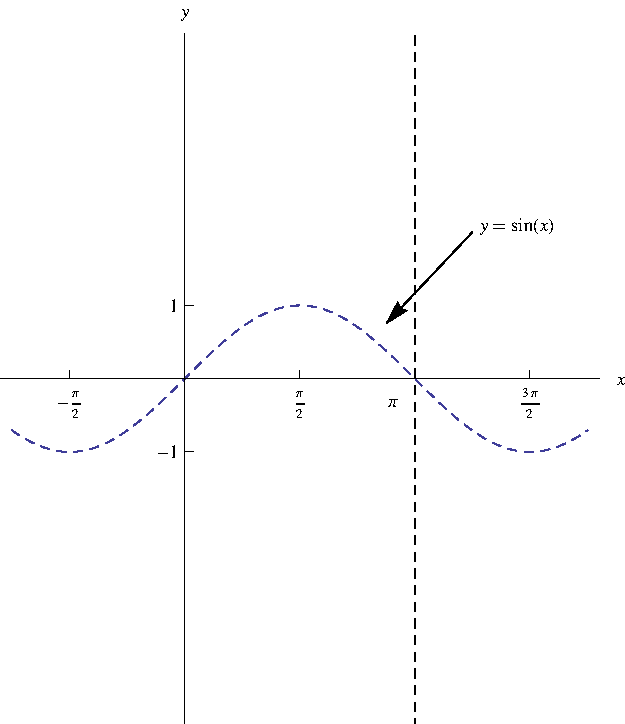
\includegraphics[width=5.5cm]{trigonometry/pictures/app-d-csca.pdf}%
%}%
%\only<2->{%
%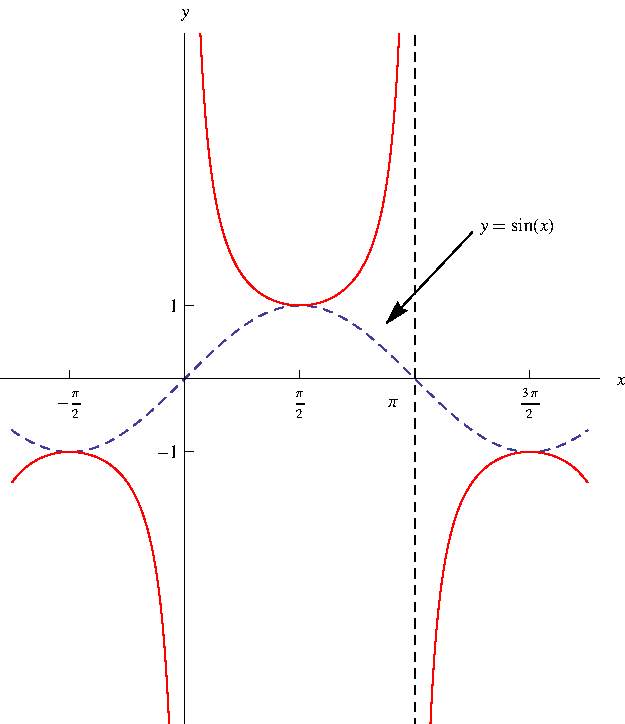
\includegraphics[width=5.5cm]{trigonometry/pictures/app-d-cscb.pdf}%
%}%

&%
\psset{xunit=0.5cm,yunit=0.5cm}
\begin{pspicture}(-4.7,-7.1)(6.1,7.1)
\psaxes[labels=none, ticks=x, Dx=1.570796327] {<->}(0,0)(-4.7,-7.1)(4.8,7.1)
\psline(-0.15, 1)(0.15,1)
\psplot[linecolor=blue!50, plotpoints=1000]{-4.7}{4.7}{x 57.295779513 mul cos}
\uncover<3->{
\psplot[linecolor=red, plotpoints=1000]{-1.420796327}{1.420796327}{1 x 57.295779513 mul cos div}
\psplot[linecolor=red, plotpoints=1000]{1.720796327}{4.56238898}{1 x 57.295779513 mul cos div}
\psplot[linecolor=red, plotpoints=1000]{-4.56238898}{-1.720796327}{1 x 57.295779513 mul cos div}
}

\psline[linestyle=dotted](1.570796327,-7.1)(1.570796327,7.1)
\psline[linestyle=dotted](-1.570796327,-7.1)(-1.570796327,7.1)
\rput[t](-3.14, -0.3){\tiny$-\pi$}
\rput[t](-1.57, -0.3){\tiny$-\frac{\pi}{2}$}
\rput[t](1.57, -0.3){\tiny$\frac{\pi}{2}$}
\rput[t](3, -0.3){\tiny$\pi$}
\rput[t](4.71238898, -0.3){\tiny$\frac{3\pi}{2}$}

\rput[bl](0.2,1){$1$}
\end{pspicture}
%\only<handout:0| -2>{%
%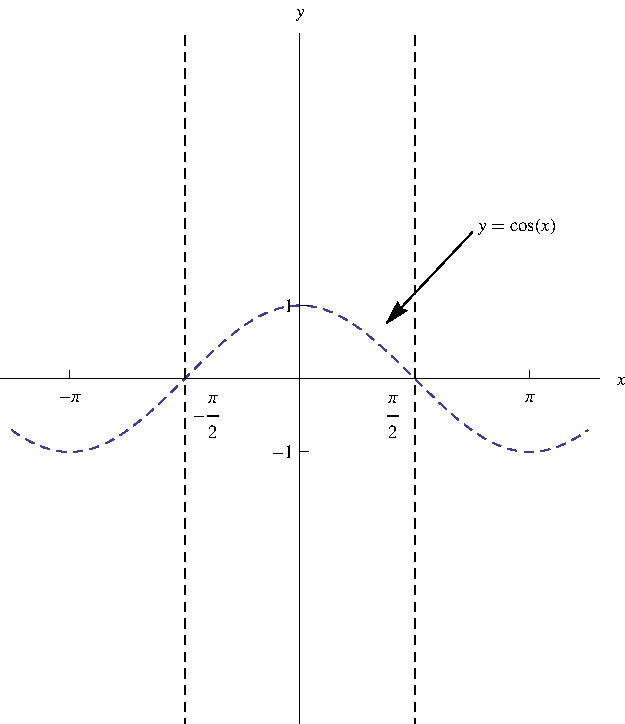
\includegraphics[width=5.5cm]{trigonometry/pictures/app-d-seca.pdf}%
%}%
%\only<3->{%
%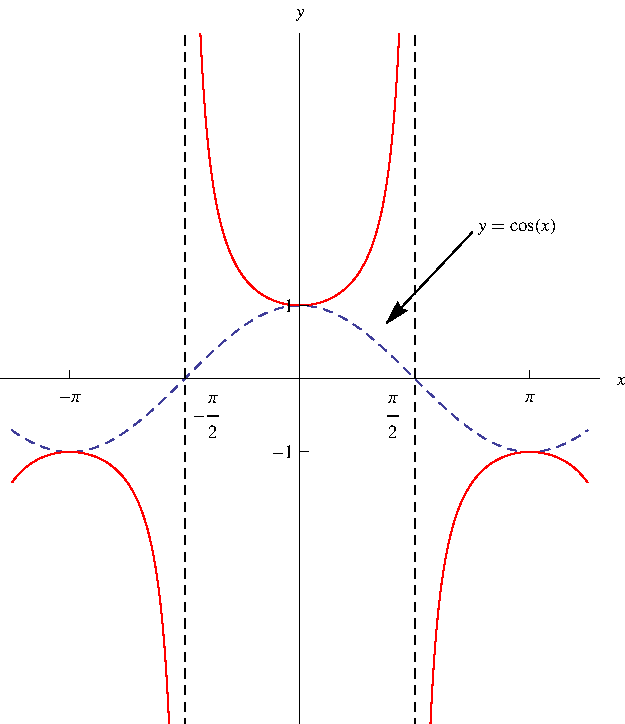
\includegraphics[width=5.5cm]{trigonometry/pictures/app-d-secb.pdf}%
%}%
\\%
$y = \csc x$  & $y = \sec x$\pause\pause\\
\end{tabular}
\end{frame}